\documentclass[a4paper,12pt]{article}
\usepackage[utf8]{inputenc}
\usepackage{amsmath,amssymb,amsthm}
\usepackage{graphicx}
\usepackage{enumerate}
\usepackage[top=1in, bottom=1in, left=1in, right=1in]{geometry}
\setlength\parindent{0pt}

\usepackage{algorithm}
\usepackage{algpseudocode}

%%%%%%%%%%%%%%%%%%%%%%%%%%%%%%%%%%%%

\usepackage{algpseudocode}% http://ctan.org/pkg/algorithmicx

\makeatletter
% This is the vertical rule that is inserted
\def\therule{\makebox[\algorithmicindent][l]{\hspace*{.5em}\vrule height .75\baselineskip depth .25\baselineskip}}%

\newtoks\therules% Contains rules
\therules={}% Start with empty token list
\def\appendto#1#2{\expandafter#1\expandafter{\the#1#2}}% Append to token list
\def\gobblefirst#1{% Remove (first) from token list
  #1\expandafter\expandafter\expandafter{\expandafter\@gobble\the#1}}%
\def\LState{\State\unskip\the\therules}% New line-state
\def\pushindent{\appendto\therules\therule}%
\def\popindent{\gobblefirst\therules}%
\def\printindent{\unskip\the\therules}%
\def\printandpush{\printindent\pushindent}%
\def\popandprint{\popindent\printindent}%

%      ***      DECLARED LOOPS      ***
% (from algpseudocode.sty)
\algdef{SE}[WHILE]{While}{EndWhile}[1]
  {\printandpush\algorithmicwhile\ #1\ \algorithmicdo}
  {\popandprint\algorithmicend\ \algorithmicwhile}%
\algdef{SE}[FOR]{For}{EndFor}[1]
  {\printandpush\algorithmicfor\ #1\ \algorithmicdo}
  {\popandprint\algorithmicend\ \algorithmicfor}%
\algdef{S}[FOR]{ForAll}[1]
  {\printindent\algorithmicforall\ #1\ \algorithmicdo}%
\algdef{SE}[LOOP]{Loop}{EndLoop}
  {\printandpush\algorithmicloop}
  {\popandprint\algorithmicend\ \algorithmicloop}%
\algdef{SE}[REPEAT]{Repeat}{Until}
  {\printandpush\algorithmicrepeat}[1]
  {\popandprint\algorithmicuntil\ #1}%
\algdef{SE}[IF]{If}{EndIf}[1]
  {\printandpush\algorithmicif\ #1\ \algorithmicthen}
  {\popandprint\algorithmicend\ \algorithmicif}%
\algdef{C}[IF]{IF}{ElsIf}[1]
  {\popandprint\pushindent\algorithmicelse\ \algorithmicif\ #1\ \algorithmicthen}%
\algdef{Ce}[ELSE]{IF}{Else}{EndIf}
  {\popandprint\pushindent\algorithmicelse}%
\algdef{SE}[PROCEDURE]{Procedure}{EndProcedure}[2]
   {\printandpush\algorithmicprocedure\ \textproc{#1}\ifthenelse{\equal{#2}{}}{}{(#2)}}%
   {\popandprint\algorithmicend\ \algorithmicprocedure}%
\algdef{SE}[FUNCTION]{Function}{EndFunction}[2]
   {\printandpush\algorithmicfunction\ \textproc{#1}\ifthenelse{\equal{#2}{}}{}{(#2)}}%
   {\popandprint\algorithmicend\ \algorithmicfunction}%
\makeatother

\begin{document}

%%%%%%%%%%%%%%%%%%%%%%%%%%%%%%%%%

% Commands


\newcommand{\setn}{\ensuremath{\{0,1\}^n}}
\newcommand{\sets}{\ensuremath{\{0,1\}^*}}
\newcommand{\zps}{\ensuremath{\mathbb{Z}_p^*}}
\newcommand{\zp}{\ensuremath{\mathbb{Z}_p}}
%%%%%%%%%%%%%%%%%%%%%%%%%%%%%%%%%

%%%%%% JAN 15

\noindent {\bf Chosen plaintext attack on NDS} \hfill January 15

Goal: find $S_k$.

Exhaustive keysearch is infeasible.  2048 bits 
$\rightarrow2^{2048}$ possible keys.

{\bf Idea:}  Let $T$ denote one round of encryption, 
i.e. takes a message in two halves
\begin{equation}\label{halves}
T(m_{i-1},m_i) - (m_i,m_{i-1} \oplus f(m_i).
\end{equation}
Let $F$ denote the encryption function.  (All 16 rounds.)

{\bf Main observation:}
$F=T^{16}$.

So, $T(F(m)) = T(T^{16}(m)) = T^{17}(m) = F(T(M))$.
i.e. $F$ and $T$ commute.

Attack: (with justification)
\begin{itemize}
\item
Fix $r\in \{0,1\}^8.$  We will determine $S_k(r)$.

\item
Select $u=(m_0,m_1)$ such that 
\begin{equation}\label{m1r}
m_1^* = r 
\end{equation}
and so 
\begin{equation}\label{n1n2}
S_{0}(n_i^j)\ne S_1(n_2^j),\quad \forall\  1\le j \le 8 
\end{equation}

\item
Obtain encryption of $u: F(u)=(a,b)$.  Then
\begin{align*}
T(F(u)) = T(a,b) &= (b,?) \quad\quad \text{by (\ref{halves})}\\
&=F(T(u))
\end{align*}
\item
Select a byte $t\in\{0,1\}^8$ and guess that $S_k(r)=t$.
\item
Apply one round of encryption to $u$, assuming that $S_k(r)=t$.
Call the result $T_t(u)$.
\item
Obtain encryption $F(T_t(u))=(c,d)$.

Note:
\begin{itemize}
\renewcommand{\labelitemii}{$\circ$}
\item
if $S_k(r)=t$, then $T_t(u)$, so $F(T_t(u)) = (b,?)$, so $b=c$.
\item
if $S_k(r)\ne t$, then $T_t(u)\ne T(u)$ by (\ref{n1n2}).
\end{itemize}
\end{itemize}
Now, if we make the heuristic assumption that $F$ behaves like a random permutation, then the probability that one would encrypt $F(T_t(u)) = F(T(u)) = (b,?)$ is
$2^{-64}$ which is negligibly small.  So if $b\ne c$ change $t$ and repeat.  Otherwise $S_k(r)=t;$ correct with high probability.

\clearpage
\noindent {\bf Chosen plaintext attack on NDS} (Continued) \hfill January 15


Attack:
\begin{algorithmic}
\Procedure{Chosen Plaintext Attack on NDS}{}
\For{$r \in \{0,1\}^8$}
	\LState 
	Select $u = (m_0,m_1)$ such that $m_1^* = r$ and 
	$S_0(n_1^j) \ne S_1(n_2^j)$ for all $j, 1 \le j \le 8$.
	\LState
	Obtain $F(u) = (a,b)$.
	\For{$t \in \{0,1\}^8$}
		\LState
		Compute $T_t(u)$
		\LState
		Obtain $F(T_t(u)) = (c,d)$
		\If{$b = c$}
			\LState
			{\bf Conclude} $S_k(r) = t$
			\LState
			{\bf goto} next $r$
		\EndIf
	\EndFor
\EndFor
\EndProcedure
\end{algorithmic}

Analysis: Expected number of chosen plaintexts is:
$$
256(1+128)\approx 2^{15} \approx 320,000 \ll 2^{2048}.
$$
Therefore NDS is {\it totally} insecure.
%%%%%%%%%% JAN 24
\clearpage
{\bf Finding collisions.} \hfill January 24

Let $H:\{0,1\}\to\setn$ be a hash function.

{\bf PROBLEM}: Find $x_1,x_2 \in \sets, x_1\ne x_2$ with $H(x_1)=H(x_2)$.

Recall the na\"ive method has run time
$$
\sqrt{\frac{\pi N}{2}}
$$
where $N=2^n$, and storage requirements
$$
\sqrt{\frac{\pi N}{2}}*2n \text{ bits.}
$$
E.g. if $n=128$, then time is $\approx 2^{64}$ steps, but the storage is $7*10^{8}$ terabytes. (About 700 billion dollars.)

{\bf Von Oorschol - Wiener (VW) collision search (1993)}

Define a sequence $\{x_i\}$ by $x_0 \in_R \setn$ and $x_i = H(x_{i-1})$,
$\forall i > 1$.  Let $y$ be the smallest index for which $x_i = x_j$ for some $i<j$.
(Such a $j$ must exist.)

Then $x_{i+\ell} = x_{j-1})$ is a collision for $H$.

By the birthday paradox,
\begin{align*}
E[j] &= \sqrt{\frac{\pi N}{2}},\\
\text{{\bf FACT}:}\quad E[i] &= \frac{1}{2}\sqrt{\frac{\pi N}{2}},\quad \text{ and}\\
E[j-i] &= \sqrt{\frac{\pi N}{2}}.
\end{align*}
{\bf MAIN IDEA}: Store {\it some} of the $x_i$'s.

Define a {\it distinguishing property} of elements of $\setn$ 
(e.g. first 10 bits are all 0).  Let $\theta$ be the proportion of elements in
$\setn$ that are distinguished.
\begin{algorithmic}

\Procedure{Stage 1}{}\label{S1} \Comment{Detecting a collision.}
	\LState
	Select distinguished point $x_0\in \setn$.
	\LState660
	Store $(x_0,0,-)$ in a table sorted by first entry.
	\LState
	$LP\gets x_0$. \Comment{$LP$ is last point stored}.
	\For{$j=1,2,\ldots$}
		\LState compute $x_j = H(x_{j-1})$.
		\If{$x_j$ is distinguished}
			\LState store $(x_j,j,LP)$.
			\LState update $LP \gets x_j$.
			\If{$x_i=x_j,i<j$}
				\LState {\bf goto} {\sc Stage 2}.
			\EndIf
		\EndIf
	\EndFor
\EndProcedure
\end{algorithmic}
\clearpage
\begin{algorithmic}
\Procedure{Stage 2}{}\label{S2} \Comment{Finding a collision, see fig. 3 handout.}
	\LState $\ell_1 \gets i-a, \ell_2 \gets j-b$.
	\LState ensure $\ell_1 \ge \ell_2$.
	\LState $k\gets \ell_1 - \ell 2$.
	\For{m=1,2,\ldots}
		\LState compute $(x_{a+k+m},x_{b+m})$
		\If{$x_{a+k+m} = x_{b+m}$}
			\LState {\bf return} $(x_{a+k+m-1},x_{b+m-1})$.
		\EndIf
	\EndFor
	
\EndProcedure
\end{algorithmic}
\begin{itemize}
\item
Analysis

Stage 1 expected time:
$$
\sqrt{\frac{\pi N}{2}} + \frac{1}{\theta}
$$
Stage 2 expected time:
$$
\frac{3}{\theta}.
$$
Expected storage:
$$
\theta + \sqrt{\frac{\pi N}{2}} (3n) \text{ bits}
$$
\end{itemize}

\clearpage
%%%%%%%%%% JAN 27

{\bf Parallelizing the VW collision finding algorithm} \hfill January 27

Given $m$-processors, run the algorithm independently on all processors.
Keep the database of distinguished points on one global server.

Expected time:
$$
\frac{1}{m} \sqrt{\frac{\pi N}{2}} + \frac{4}{\theta}
$$
Space: 
$$
\theta + \sqrt{\frac{\pi N}{2}} (3n) \text{ bits}
$$
(same).

Note: the processors do not communicate with each other.  They only occasionally communicate with the central server.
\\[2em]
{\bf Finding meaningful collisions.}

Let $m_1$ and $m_2$ be arbitrary messages.  We'll show how $A$ (the VW algorithm)
can be used to find modifications $\hat m_1$ and $\hat m_2$ of $m_1$ and $m_2$ 
so that $H(\hat m_1) = H(\hat m_2)$ and $\hat m_1$ and $\hat m_2$ have the same
meaning as $m_1$ and $m_2$, respectively.
The new algorithm will have the same run-time as well.

\begin{itemize}
\item
Define $g_{m_1}:\setn \to \sets$ as follows:

Fix $n$ positions in $m_1$, say $j_1,\ldots, j_n$ (e.g. the ends of sentences). 
Then for $r\in \setn$, define $g_{m_1}(r)$ to be the message obtained from $m_1$
by adding for each $1\le i \le n$ a space at position $j_i$. iff the $i$-th bit
of $r$ is 1.  Note $g_{m_1}(r)$ has the same meaning as $m_1$.
\item
Define $g_{m_2}$ in the same way.
\item
Partition $\setn$ into 2 sets $S_1$ and $S_2$ of the same size.
\item
Define $f:\setn\to\setn$ as follows:
$$
f(r) =
\begin{cases}
H(g_{m_1}(r)) \text{ if } r\in S_1 \\
H(g_{m_2}(r)) \text{ if } r\in S_2
\end{cases}
$$
If $H$ is viewed as a random function, then so is $f$.

{\bf Attack}: Run $A$ on $f$.

$A$ will produce a collision $(a,b)$.  Suppose $a$ and $b$ are from different sets $S_1$ and $S_2$, i.e. $a\in S_1$, $b\in S_2$.  Then
$$
f(a)=H(g_{m_1}(a)) = H(g_{m_2}(b)).
$$
Letting $\hat m_1 = g_{m_1}(a), \hat m_2 = g_{m_2}(b)$, we have $H(\hat m_1) = H(\hat m_2)$

\end{itemize}

%%%%%% JAN 29

\clearpage
{\bf Iterated Hash Functions}\hfill January 29

Ingredients:
\begin{itemize}
\item
Compression function $f:\{0,1\}^{n+r} \to \setn$.
\item
Initialization vector $\text{\sc iv} \in\setn$.
\end{itemize}
To hash $x\in\sets$, do:
\begin{itemize}
\item
Break $x$ into $r$-bit blocks: $\hat x = x_1,\ldots,x_t$,
where $x_t$ is padded with zeros if necessary.
\item
Let $b$ be the bit length of $x$.
\item
Let $x_{t+1}$ be the (right-justified) binary representation of $b$.
\item
So $H:\sets \to \setn$.
\end{itemize}

{\bf Theorem:} (Merkel) If $f$ is collision resistant, then $H$ is collision resistant.

\begin{proof}
Suppose $H$ is not collision resistant.  Then we have an efficient algorithm which finds a collision for $H$.  We use the algorithm to find a collision for $H$; $(x,x')$.  Write:
\begin{align*}
\hat x &= x_1, x_2, \ldots, x_t, b = \text{ bitlength of }x, x_{t+1}, \text{length block of }x\\
\hat x' &= x_1', x_2', \ldots, x_t', b' = \text{ bitlength of }x', x'_{t+1}, \text{length block of }x'\\
\end{align*}
Now, efficiently compute
\begin{align*}
H_0 &= \text{\sc iv} & H_0'&= \text{\sc iv}\\
H_1 &= f(H_0,x_1) & H_1 &= f(H_0,x_1)\\
&\vdots&\vdots&\\
H_t &= f(H_{t-1},x_t)&H_t &= f(H_{t-1},x_t)\\
H_{t+1} &= f(H_t,x_{t+1})&H_{t+1} &= f(H_t,x_{t+1})\\
\end{align*}
So $H(x) = H(x')$

If $b\ne b'$ then $x_{t+1}\ne x'_{t'+1}$.  So $((H_t,x_{t+1}),(H'_{t'},x'_{t'+1}))$
is a collision for $f$.

If $b=b'$ then $t=t'$.  Then $H_t,H'_{t'}$ might be a collision if they are not equal.  If they are equal, try $(H'_{t-1},H'_{t'-1})$.  The collision is the largest $i$ such that
$(H_i,x_{i+1})\ne (H'_i,x'_{i+1})$ but $f(H_i,x_{i+1})=f(H'_i,x'_{i+1})$.
\end{proof}
%%% FEBRUARY 5
\clearpage

\noindent {\bf Using a MAC Scheme for Non-Repudiation} \hfill February 5

A MAC Scheme and trusted third party can be used to verify that Alice signed a message:
\begin{enumerate}
\item Alice shares a key $k_{AT}$ with a trusted third party (TTP).
\item Alice sends $(x, \text{MAC}_{k_{AT}}(x))$ to Bob.
\item Bob asks the TTP to verify the signed message.
\item In case of a dispute, the judge asks the TTP to verify the signed message.
\end{enumerate}

%%% FEBRUARY 12
\clearpage
\noindent {\bf Basic RSA Encryption Scheme} \hfill February 12

{\bf Key Generation.}
\begin{enumerate}
\item Randomly select $p,q$ distinct large primes of bitlength $k \ge 512$.
\item Compute $n = pq$ and $\varphi(n) = (p-1)(q-1)$.
\item Select $e \in [1,\varphi(n)]$ with $\gcd(e,\varphi(n))=1$.
\item Compute $d = e^{-1} \mod \varphi(n)$.
\item Public key is $(n,e)$ and private key is $d$.
\end{enumerate}

{\bf Encryption.}
\begin{enumerate}
\item Obtain an authentic copy of Bob's public key, $(n,e)$.
\item Represent the message as an integer $m \in [0,n-1]$.
\item Compute $c = m^e \pmod n$.
\item Send $c$ to Bob.
\end{enumerate}

{\bf Decryption.}
\begin{enumerate}
\item Compute $m = c^d \mod n$.
\end{enumerate}

{\bf Proof that RSA Decryption Works.}
Since $ed \equiv 1 \pmod{\varphi(n)}$, we can write $ed = 1+k\varphi(n)$ for some $k \in \mathbb{Z}$. If $m \equiv 0 \pmod{p}$, then $m^{ed} \equiv 0 \pmod{p}$, so $m^{ed} \equiv m \pmod{p}$. If $m \not\equiv 0 \pmod{p}$, then $m^{p-1} \equiv 1 \pmod{p}$ (by Fermat). Thus $m^{k(p-1)(q-1)} \equiv 1 \pmod{p}$ and thus $m^{k(p-1)(q-1)+1} \equiv m \pmod{p}$. Thus $m^{ed} \equiv m \pmod{p}$. Similarly $m^{ed} \equiv m \pmod{q}$, so $m^{ed} \equiv m \pmod{n}$, since $p$ and $q$ are distinct primes.

\vspace{1cm}

\noindent {\bf Basic RSA Signature Scheme}

{\bf Signature Generation.}
\begin{enumerate}
\item Compute $M=H(m)$ where $H$ is a hash function.
\item Compute $s=M^d \pmod n$.
\item Send message-signature pair $(m,s)$.
\end{enumerate}

{\bf Signature Verification.}
\begin{enumerate}
\item Obtain an authentic copy of public key $(n,e)$.
\item Compute $M'=H(m)$
\item Accept message if $s^e \equiv M' \pmod n$.
\end{enumerate}

%%%%%%%%% FEB 14
\clearpage
{\bf Security of RSA}\hfill February 14

\begin{enumerate}[I.]
\item
Key generation
\item
Encryption
\item
Signatures
\end{enumerate}

\begin{enumerate}
\item[I.]
{\bf Key Generation}

Given a public key $(n,e)$, can an adversary obtain the private key $(n,d)$?
\begin{itemize}
\item
{\sc compute}-$d$: given $(n,e)$, compute $d$.
\item
{\sc factor}: given $(n,e)$, compute $p$ and $q$.
\item
{\sc compute}-$\varphi(n)$: given $(n,e)$, compute $\varphi(n)$.
\end{itemize}
Definition: Let $A_1$ and $A_2$ be two computational problems.  We say that $A_1$ {\it polynomial time reduces to} $A_2$, written $A_1 \le_p A_2$ if there is a polynomial time algorithm for solving $A_1$ which uses a polynomial time oracle for solving $A_2$.  If $A_1 \le_p A_2$ and $A_2 \le_p A_1$ then we say $A_1$ and $A_2$ are {\it computationally equivalent} and write $A_1 \equiv_p A_2.$

E.g. {\sc compute}-$\varphi(n)$ $\le_p$ {\sc factor}.
\begin{proof}
We are given an oracle for {\sc factor} and an instance $(n,e)$ of {\sc compute}-$\varphi(n)$.  We need to compute $\varphi(n)$.  We give $(n,e)$ to {\sc factor} to obtain $p,q$.  Now we can compute $\varphi(n)=(p-1)(q-1)$.  All of this is done in polynomial time.
\end{proof}
{\bf Fact:} {\sc factor} $\le_p$ {\sc compute}-$d$.
\end{enumerate}

%%%%%%%%% FEB 14
\clearpage
{\bf Security of RSA continued}\hfill February 24

\begin{enumerate}
\item[II.]
{\bf Encryption}
\begin{itemize}
\renewcommand{\labelitemii}{$\circ$}
\item
What does it mean for RSA encryption to be secure?
\item
{\sc rsap:} Given $(n,e)$ and $c$, find $m\in [0,n-1]$ such that $c=m^e\pmod n$.
\item
Clearly {\sc rsap} $\le_p$ {\sc factor}.  Does {\sc factor} $\le_p$ {\sc rsap}?
This is a big question.
\item
Chosen ciphertext attack on RSA encryption:
\begin{itemize}

\item
$E$ is given $(n,e)$ and target ciphertext $c=m^e \pmod n$.
\item
$E$ has access to a decryption oracle, to which $E$ can present any ciphertext except $c$ itself.
\end{itemize}
{\bf} Attack:
\begin{enumerate}[(i)]
\item
$E$ selects arbitrary $x\in [2,n-1]$ with $\gcd(x,n)=1$.
\item
$E$ computes $\hat c = cx^e \pmod n$ and presents $\hat c$ to the decryption oracle which returns $\hat m = \hat c^d \pmod n$.

Note: $\hat m = \hat c^d = (cx^e)^d = c^dx^{ed} = mx \pmod n$.
\item
$E$ computes $m=\hat m x^{-1} \pmod n$.
\end{enumerate}
\item
To circumvent the attack, Alice adds some ``structure" to $m$ prior to decryption.  Now, if a ciphertext is decrypted by Alice and the resulting plaintext does not have the required structure, the ciphertext is rejected.
\item
Forward search attack on basic RSA encryption:
\begin{itemize}
\item
Suppose the plaintext space is small or easily predictable.
\item
$E$ can build a dictionary of $(PT,CT)$ pairs and then compare the transmitted ciphertext with the ones in the dictionary.
\item
To circumvent the attack, the plaintext is ``salted'', i.e. a random string of length 128 bits (say) is appended to $m$ prior to encryption.
\end{itemize}
\end{itemize}

\end{enumerate}
%%%%%%%% FEB 26
\clearpage
{\bf Security of RSA continued}\hfill February 26
\begin{itemize}\renewcommand{\labelitemii}{$\circ$}
\item
Definition: a public key encryption scheme is {\it secure} if it is symantically secure against chosen ciphertext attack, by computationally bounded adversary.
\item
Basic RSA is {\it insecure}.
\item
In practice RSA PKCS \#1 V1.5 is used.
\begin{itemize}
\item
Encryption: $M \mapsto m \mapsto c=m^e \pmod m$, where $m$ is the formatted version of $M$.
\item
Decryption: $c \mapsto m = c^d \pmod n \mapsto M$, where we check and remove the formatting of $m$ to obtain $M$.
\end{itemize}
\item
Let $k$ be the bitlength of $n$ (e.g. $k=128$).
\item
Formatting:
\begin{center}
\begin{tabular}{|c|c|c|c|c|}
\hline
00 & 02 & $xxx \ldots xxx$ & 00 & M\\
\hline
\end{tabular}
\end{center}
\item
{\bf Problem:} RSA PKCS \#1 V1.5 is {\it not} secure.
\item
Blerchenbacher (1998) ``restricted'' chosen-ciphertext-attack on RSA PKCS \#1 V1.5.
\item
Suppose $c$ is the target ciphertext.  The adversary can carefully select about 500,000 variants $c'$ of $c$ and presents $c'$ to the decryption.  The decryptor lets the adversary know if the corresponding plaintext is formatted correctly or not.
\item
Also used is RSA-OAEP (PKCS\#1 V2).  RSA-OAEP is {\it secure}.
\end{itemize}


%%% FEBRUARY 28
\clearpage
{\bf Security of RSA continued} \hfill February 28
\begin{enumerate}
\item[III.]
{\bf RSA PKCS \#1 V1.5 Signature Scheme}

{\bf Signature Generation.}
Alice does:
\begin{enumerate}
\item Compute $h = H(m)$, where $H$ is a hash function.
\item Format $h$ as follows where $k$ is the bytelength of $n$
\[
M = \underbrace{{\tt 0001FFFF\cdots FF00\overbrace{xxxx\cdots xx}^{\substack{\text{hash name}\\15\text{ bytes}}}h}}_{k\text{ bytes total}}
\]
\item Compute $s = M^d \mod n$.
\item The signed message is $(m,s)$.
\end{enumerate}

{\bf Signature Verification.}
Bob does:
\begin{enumerate}
\setcounter{enumi}{-1}
\item Obtain an authentic copy of Alice's public key.
\item Compute $M = s^e \mod n$.
\item Check the formatting of $M$:
\begin{itemize}
\item Write $M$ as a bytestring of length $k$.
\item Check:
\begin{itemize}
\item 1st byte is {\tt00}
\item 2nd byte is {\tt01}
\item Next bytes are {\tt FF} bytes followed by a {\tt00} byte.
\end{itemize}
\end{itemize}
\item Extract hash name from next 15 bytes.
\item Extract $h$ from the remaining bytes (length based on hash function) and check there are no extra bytes at the end.
\item Accept iff $h = H(m)$.
\end{enumerate}

{\bf Breaking RSA PKCS \#1 V1.5 Signatures by Hand.}

Assumptions:
\begin{enumerate}
\item $e=3$ (this is widely used).
\item Verifier does not check for extra ``garbage'' bytes at end of $M$. (In 2006: OpenSSL, Firefox 2, Sun's JRE, Adobe Acrobat, etc did not check.)
\item $H = \text{SHA-1}$ (WLOG)
\item $n$ is 3072 bits (WLOG)
\end{enumerate}

Attack:
\begin{enumerate}
\item Select any $m$.
\item Compute $h = H(m)$.
\item Let $D = {\tt 00\underbrace{xxxx\cdots xx}_{\text{hash name}}}h$
\item Let $N = 2^{288}-D$ and assume that $3 \mid N$ (if not, modify $m$ and repeat).
\item Let $s = 2^{1019}-2^{34}N/3$.
\end{enumerate}

\emph{Claim:} $(m,s)$ is accepted by the verifier.

\emph{Proof:}
\begin{align*}
s^3 &\equiv (2^{1019}-2^{34}N/3)^3 \mod n  \\
&= 2^{3057}-2^{2072}N+\underbrace{\frac{2^{1037}N^2}3 - \left(\frac{2^{34}N}{3}\right)^3}_{\text{garbage }<2^{2072}} \\
&= 2^{3057} - 2^{2072}(2^{288}-D) + \text{garbage} \\
&= 2^{3057} - 2^{2360} + 2^{2072}D + \text{garbage} \\
&= 2^{2360}(2^{697}-1)+2^{2072}D + \text{garbage}
\end{align*}
\[
M_{\text{hex}} = {\tt 0001}\underbrace{\tt FFFFFF\cdots FF}_{\text{696 bits}}\underbrace{{\tt 00}xxxx\cdots xx}_{\text{288 bit }D} \underbrace{yyyyyy\cdots yy}_{\text{2071 bit garbage}}
\]
\end{enumerate}

%%%%%%%%%% MAR 7
\clearpage
{\bf Math background for discrete logs}\hfill March 7, 2014

Background in number theory:
\begin{itemize}
  \item
  Let $p$ be a prime.
  \item
  $\mathbb{Z}_p = \{ 0,1,\ldots, p-1\}$ with addition
  done modulo $p$.
  \item
  $\mathbb{Z}_p^* = \{0,1,\ldots,p-1\}$. (All integers
  relatively prime to $p$ i.e. all of them)
  \item
  Fermat's Little Theorem:
  
  If $p$ is prime and $a\in \mathbb{Z}_p^*$ then
  $a^{p-1} = 1 \pmod p$.
  \item
  Definition: Let $P$ be prime, and $a\in\mathbb{Z}^*_p$
  The {\it order} of $a$, denoted $\text{ord}(a)$ is the
  smallest positive integer $t$ such that
  $a^t\equiv 1 \pmod p$.
  
  e.g. Let $p=13.$  In $\mathbb{Z}_{13}:$
  \begin{align*}
   \text{ord}(1)&=1\\
   \text{ord}(3)&=3\\
   \text{ord}(12)&=2\\
   \text{ord}(2)&=12
  \end{align*}
  \item
  {\bf Facts.}
  Let $p$ be prime, $a\in\mathbb{Z}_p^*$, and suppose
  $ord(a)=t.$
  \begin{enumerate}
   \item Let $r\in \mathbb{Z}.$ Then $a^r \equiv 1 \pmod p$
   iff $t|r$.
   \item
   $t|p-1$
   \item
   Let $x,y\in\mathbb{Z}$.  Then $a^x\equiv a^y$ iff
   $x\equiv y \pmod t$.
   \item
   If $r\in\mathbb{Z}$ then $a^r\equiv a^{r\pmod t} \pmod p$.
  \end{enumerate}
\item
Definition.  Let $p$ be a prime.
Then $a\in\mathbb{Z}_p^*$ is
a {\it generator} of $\mathbb{Z}_p^*$ if $\text{ord}(a)=p-1$.  
Then $\{a^i \pmod p : 0\le i \le p-2\} = \mathbb{Z}_p^*$.
\end{itemize}
\clearpage
%%%% March 10

{\bf Discrete Logarithm (DL) public-key systems}\hfill March 10

\begin{itemize}
 \item 
 Security is based on hardness of discrete log problem.
 \item
 Let $p,q$ be primes with $q|(p-1)$.  Let $g$ be an element of order $q$ in \zps.
 \item
 Such an element $g$ exists:
 
 Let $\alpha$ be a generator of \zps.  Then let $g=\alpha^{(p-1)/q}\pmod p$.
 Then $g^q = \alpha^{p-1} \equiv 1 \pmod p$, so ord$(g)|q$.  
 Since $q$ is prime, and ord$(g)\ne 1$, we have ord$(g)=q$.
 \item
 Definition: $\langle g \rangle = \{q^i \pmod p : a < i \le q-1 \}$, or the
 {\it subgroup of \zps generated by $g$.}
 \item
 E.g. Take $p=67$, $q=11$, $g=9$.
 \begin{align*}
 9^0 \equiv 1 & & 9^3 \equiv 59 && 9^6 \equiv 64 & & 9^9 \equiv 24 \\
 9^1 \equiv 9 & & 9^4 \equiv 62 && 9^7 \equiv 40 & & 9^{10} \equiv 15\\
 9^2 \equiv 14 && 9^5 \equiv 22 && 9^8 \equiv 25 & & 9^{11} \equiv 1\\
 \end{align*}
So ord$(9)=11$.

What power of 9 gives 25 modulo 67?  Answer: 8, i.e. $8=\log_9 25$.
\end{itemize}
{\bf Discrete Log Problem (DLP)}

Given $p,q,g$ and $h\in \langle g \rangle$, find the integer $a\in [0,q-1]$ such that
$h\equiv g^a \pmod p$.  We write $a=\log_g h$ (in \zps).

Note:
\begin{itemize}
 \item $\log_g(h_1h_2)\equiv \log_g(h_1) + \log_g(h_2)\pmod q$.
 \item $\log_g(h_1^c)=c\log_g(h_1) \pmod q$.
\end{itemize}

{\bf Fastest known algorithms for DLP}
\begin{enumerate}
 \item Exhaustive search
 
 Compute $g^0,g^1,\ldots \pmod p$ until you encounter $h$.
 
 Runtime: $\mathcal O (q)$ modulo multiplications.
 
 \item Shanks' algorithm
 
 {\bf Idea:} Let $m=\lceil \sqrt q \rceil$.  Write $a=im+j$ where
 $0\le j \le m-1$ and $0\le i \le m-1$.  Notice that $i$ and $j$ are unique.
 
 Then $h\equiv g^a \equiv g^{im+j} \pmod p$, so
 $$
 g\cdot (g^{-m})^i \equiv g^j \pmod p
 $$
 Same idea as meet in the middle attack on double DES ($c = DES_{k_2}(DES_{k_1}(m))$)
 
 Algorithm:
 
 1. Compute $g^j \pmod p$ for $j=0,..,m-1$.\\
    Store $(g^j \pmod p, j)$ in the table, sorted by first entry\\
 2. Compute $g^m \pmod p$ and $t=g^{-m} \pmod p$\\
 3. For $i=0,1,\ldots$ compute $h\cdot t^q \pmod p$.  
    If this is in the table, say $ht^i=g^j \pmod p$ then
    $\log_gh=im+j$.  STOP.
 
 Runtime: $\mathcal O (\sqrt{q})$ modular multiplications.
 
 Storage: $\mathcal O (\sqrt q)$.
 
 \item
 Pollard's Algorithm:
 
 Runtime: $\mathcal O (\sqrt q)$ modular multiplications.
 
 Storage: negligible.
 
\item
 NFS.
 
 Runtime $L_p [\frac{1}{3},1.923]$.  
 
 Recall that runtime of NFS for factoring $n$ is $L_p [\frac{1}{3},1.923]$.

\end{enumerate}
\begin{itemize}
 \item[E.g.]
For an 80-bit security leevel, we need $p\approx2^{1024}$ 
and $q\approx 2^{160}$.
(see runtim for NFS factoring.)
\item[E.g.]
For a 128-bit security level, we need $p\approx 2^{3072}$ and $q\approx 2^{256}$.
\end{itemize}

Next time:
\begin{enumerate}
 \item Diffie-Hellman key agreement.
 \item Digital Signature Algorithm (DSA).
\end{enumerate}

\clearpage

%%%% MARCH 14

{\bf Diffe-Hellman (DH) Key Agreement Scheme } (1975)
\hfill
March 14

{\bf Purpose}: Two parties to agree upon a shared secret key.

{\bf Domain parameters (public)}: $p,q,g$ such that $p$ and $q$ are primes, $q \mid p-1$, $q \in \mathbb{Z}_p^*$ with $\text{ord}(g) = q$. (For example, for 80-bit security, one might use a 160-bit $q$ and 1024-bit $p$.

{\bf Unauthenticated DH}:
\begin{enumerate}[1.]
\item Alice selects $x \in_R [1,q-1]$ and computes $X = g^x \mod p$ and sends $X$ to Bob.
\item Bob selects $y \in_R [1,q-1]$ and computes $Y = g^y \mod p$ and sends $Y$ to Alice.
\item Alice computes $K = Y^x \mod p = g^{yx} \mod p$ and Bob computes $K = X^y \mod p = g^{xy} \mod p$. Both Alice and Bob have the same $K$.
\item The shared secret key is $k = H(K)$.
\end{enumerate}
An eavesdropper is faced with the following problem:
\begin{quote}
\emph{Diffe-Hellman Problem (DHP)}: Given $p,q,g,g^x \mod p, g^y \mod p$, compute $g^{xy} \mod p$.
\end{quote}
Clearly DHP $\le_P$ DLP. It is conjectured that DLP $\le_P$ DHP.

{\bf Person-in-the-middle attack}: The attacker:
\begin{itemize}
\item Chooses $x',y'$. 
\item Intercepts Alice's $X$ and sends her $Y' = g^{y'} \mod p$. Alice then computes $K_1 = g^{xy'} \mod p$. The attacker can also compute $K_1$.
\item Intercepts Bob's $Y$ and sends him $X' = g^{x'} \mod p$. Bob then computes $K_2 = g^{yx'} \mod p$. The attacker can also compute $K_2$.
\item Intercepts a message from Alice, decrypts it using $K_1$, reads it, encrypts it using $K_2$, and sends it to Bob. The attacker can read the messages sent from Alice to Bob without them knowing. (A similar process works for messages sent from Bob to Alice.)
\end{itemize}

{\bf Authenticated DH}:
\begin{itemize}
\item Alice sends Bob $(X,\text{``Alice''})$.
\item Bob then sends Alice $(Y, \text{Sign}_\text{Bob}(Y,X,\text{``Alice''}))$. ($\text{Sign}_\text{Bob}$ denotes Bob's RSA signature.)
\item Alice then verifies Bob's signature on $(Y,X,\text{``Alice''}))$ and sends to Bob \\$\text{Sign}_\text{Alice}(X,Y,\text{``Bob''})$. ($\text{Sign}_\text{Alice}$ denotes Alice's RSA signature.)
\end{itemize}

\clearpage
{\bf Digital Signature Algorithm (DSA)} (1991)
\hfill
March 14

(Standardized by US government in 1993.)

{\bf Domain parameters (public)}: $p,q,g$ such that $p$ and $q$ are primes, $q \mid p-1$, $q \in \mathbb{Z}_p^*$ with $\text{ord}(g) = q$.

{\bf Key Generation}: Alice does
\begin{enumerate}[1.]
\item Select $a \in_R [1,q-1]$.
\item Compute $h = g^a \mod p$.
\item Alice's private key is $a$ and her public key is $h$.
\end{enumerate}

{\bf Signature Generation}: To sign $M \in \{0,1\}^*$, Alice does:
\begin{enumerate}[1.]
\item Compute $m = H(M)$.
\item Select a {\em per-message secret} $k \in_R [1,q-1]$.
\item Compute $r = (g^k \mod p) \mod q$ and check that $r \ne 0$.
\item Compute $s = k^{-1}(m+ar) \mod q$ and check that $s \ne 0$.
\item Alice's signature on $M$ is $(r,s)$.
\end{enumerate}

%%%% MARCH 17

\clearpage
{\bf Digital Signature Algorithm (DSA) Continued}
\hfill
March 17\\[0.5em]

{\bf Signature Verification}: To verify $M, (r,s)$, Bob does:
\begin{enumerate}[1.]
\item Obtain an authentic copy of Alice's public key $h$.
\item Verify that $1 \le r,s \le q-1$.
\item Compute $m = H(M)$.
\item Compute $u_1 = s^{-1}m \mod q$ and $u_2 = s^{-1}r \mod q$.
\item Compute $v = (g^{u_1}h^{u_2} \mod p) \mod q$.
\item Accept iff $v = r$
\[
\text{Idea: }s \equiv k^{-1}(m+ar) \pmod q \iff k \equiv s^{-1}(m+ar) \pmod q \iff g^k \equiv g^{s^{-1}(m+ar)} \pmod p 
\]\[
\iff g^k \equiv g^{s^{-1}m}h^{s^{-1}r} \pmod p \Rightarrow \underbrace{(g^k \mod p) \mod q}_r = \underbrace{(g^{s^{-1}m}h^{s^{-1}r} \mod p) \mod q}_v
\]
\end{enumerate}

{\bf Security Notes}:
\begin{enumerate}[1.]
\item DSA is {\em believed} to be {\em secure}, assuming DLP is hard and $H$ is ``secure''.
\item $k$ should be securely destroyed after it is used.
\item $k$ should never be reused.
\item Finding $M$ such that $H(M) = 0$ should be infeasible. [See assignment 4.]
\end{enumerate}

{\bf DSA vs RSA Signature Schemes at 128-bit security level}:
\begin{itemize}
\item For RSA with 128-bit security, we need $n$ to be 3072 bits. \\
For DSA with 128-bit security, we need $p$ to be 3072 bits and $q$ to be 256 bits.
\item {\em Signature Size}: RSA signatures are 3072 bits, whereas DSA signatures are 512 bits. Thus, DSA signatures are better in applications where small signatures are required.
\item {\em Speed}: \\
RSA: In practice, $e = 3$ or $e = 2^{16} + 1$ so signature verification is fast. However, signature generation is slow, but one could not speed it up by choosing a small $d$, because this would make the scheme insecure. \\
DSA: In signature generation, $k, r, k^{-1}, k^{-1}ar$ can be computed before one knows $M$. Signing then requires computation of $m = H(M)$ and
$s = k^{-1}(m + ar)$. So signature generation is fast.
\end{itemize}

\clearpage
{\bf Elliptic Curve Cryptography}
\hfill
March 17 \\

{\bf Idea:}
Replace $\langle g \rangle$ with the group of points on an elliptic curve. \\

{\bf Definition.}
Let $F = \mathbb{R}$ or $\mathbb{Z}_p$ (where $p \ge 5$ is prime). An elliptic curve over $F$ is defined by an equation $Y^2 = X^3 + aX + b$ where $a,b \in F$ and $4a^3 + 27b^2 \ne 0$. The points on $E$ is $E(F) = \{(x,y) : y^2 = x^3 + ax + b, \hspace{2mm} x,y \in F\} \cup \{\infty\}$ where $\infty$ is the point at infinity. \\

{\bf Examples.}

\begin{figure}[h!]
\begin{minipage}{0.45\textwidth}
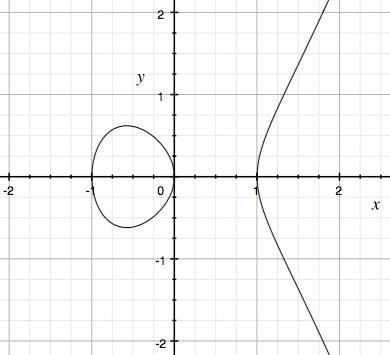
\includegraphics[width=\textwidth]{fig-mar17-1}
\caption{$E: Y^2 = X^3 - X$ over $\mathbb{R}$}
\end{minipage}
\hspace{0.05\textwidth}
\begin{minipage}{0.45\textwidth}
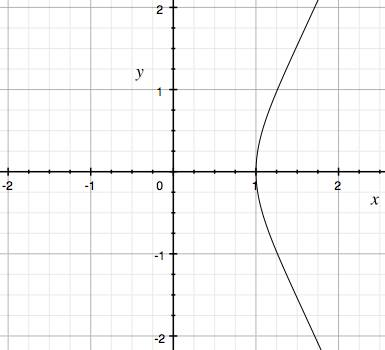
\includegraphics[width=\textwidth]{fig-mar17-2}
\caption{$E: Y^2 = X^3 - 1$ over $\mathbb{R}$}
\end{minipage}
\end{figure}

{\bf Example.}
$E: Y^2 = X^3 + 2X + 9$ over $\mathbb{Z}_{13}$. The points on $E$ are:
\[
E(\mathbb{Z}_{13}) = \{(0,3),(0,10),(1,5),(1,8),(3,4),(3,9),(4,4),(4,9),(5,1),(5,12),(6,4),(6,9),(8,2),
\]\[
(8,11),(11,6),(11,7),\infty\}
\]
\clearpage
{\bf Elliptic Curves Continued}  \hfill March 19
\\[1em]
{\bf Number of points in $E(\zp)$}
\\[1em]
Clearly, $1\le \# E(\zp)\le 2p+1$.  In fact,
$(\sqrt p -1)^{2} \le E(\zp)\le (\sqrt p +1)^{2}$.
(Hasse's Theorem).
Hence $\#E(\zp)\approx p$.
\\[1em]
There is a natural way to add two points in $E(F)$ to get
a third point in $E(F)$.
\begin{figure}[h!]
\centering
\begin{minipage}{0.45\textwidth}
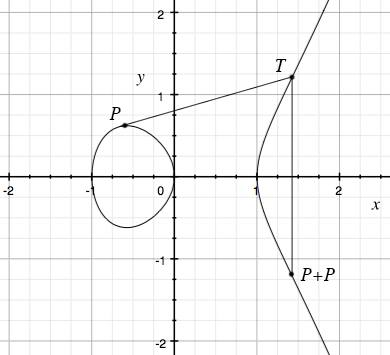
\includegraphics[width=\textwidth]{fig-mar19-1}
\caption{$P+Q$}
\end{minipage}
\hspace{0.05\textwidth}
\begin{minipage}{0.45\textwidth}
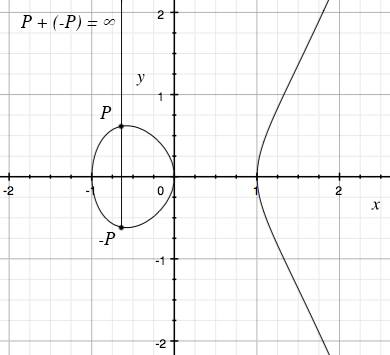
\includegraphics[width=\textwidth]{fig-mar19-2}
\caption{$P+(-P)$}
\end{minipage}
\hspace{0.05\textwidth}
\begin{minipage}{0.45\textwidth}
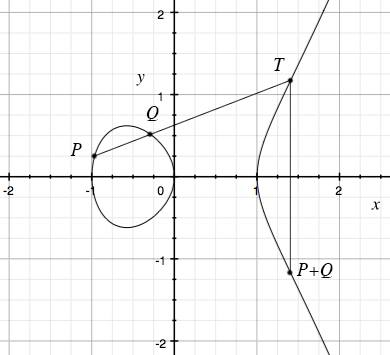
\includegraphics[width=\textwidth]{fig-mar19-3}
\caption{$P+P$}
\end{minipage}
\hspace{0.05\textwidth}
\end{figure}


{\bf Algebraic formulas for point addition in $E(F)$
($F=\mathbb{R}$ or $F=\zp$)}

\begin{enumerate}
\item
$P+\infty = P = \infty + P,\quad \forall P \in F$.
\item
If $P = (x,y)$ and $Q = (x,-y)$ then $P+Q=\infty$.
Here, we write $Q = -P$.  Therefore $\infty = - \infty$.
\item
If $P=(x_1,y_1)$, $Q=(x_2,y_2)\in E(F)$, $P\ne \pm Q$,
then $P+Q = (x_3,y_3)$, where

$\ell : y=y_1 + \lambda(x-x_1)$, $\lambda = \frac{y_2 - y_1}{x_2-x_1}$.
Substitute for $y$ in $y^2 = x^3 + ax + b$:

$x^3+ax + b - (y_1 + \lambda(x-x_1))^2 = 0 = (x-x_1)(x-x_2)(x-x_3)$.

Equate coefficients of $x^2$:
\begin{align*}
-\lambda^2 &= -x_1 - x_2 - x_3 \\
x_3 &= \lambda^2 - x_1 - x_2.
\end{align*}
The $y$-coordinate of $T$ is $y_3 = y_1 + \lambda (x_3 - x_1)$.
So the $y$-coordinate of $R$ is $y_3 = -y_3'$.
\begin{align*}
x_3 &= \lambda^2 - x_1 - x_2, 
&\text{where } \lambda = \frac{y_2-y_1}{x_2-x_1}\\
y_3 &= -y_1 + \lambda(x_1-x_3)
\end{align*}
\item
If $P - (x_1,y_1)$, $P\ne -P$, then $P + P = 2P = (x_3,y_3)$ where
\begin{align*}
x_3 &= \lambda^2 - 2x_1 
\text{ where } \lambda = \frac{3x_1^2 + a}{2y_1}\\
y_3 &= -y_1 + \lambda (x_1 - x_3)
\end{align*}
Here, $\lambda$ is obtained from partial derivatives of $y^2 = x_3 + ax +b$.
\end{enumerate}
{\bf Addition in $E(F)$ has the following properties}
\begin{enumerate}
\item
$P+\infty = \infty + P = P,\quad\forall P \in E(F)$.
\item
For each $P\in E(F),\quad \exists Q \in E(F)$ such that $P+Q = \infty$.
\item
$P+Q = Q+P,\quad \forall P,Q \in E(F)$.
\item
$P+(Q+R)=(P+Q)+R,\quad\forall P,Q,R \in E(F)$ (needs proof).
\item[]
That is, $E(F)$ is an {\it Abelian group.}
\end{enumerate}
{\bf Elliptic curve discrete log problem ({\sc ecdlp})}
\\[1em]
$E=$ elliptic curve over \zp,
$q=\#E(\zp), P\ne \infty$, and suppose $q$ is prime.
Then $\{ P, 2P, 3P, \ldots, qP \} = E(\zp)$.
\\[1em]
{\sc ecdlp}:

Given $p,E,q, P$ and $Q \in E(\zp)$, find $\ell \in [ 0, q-1]$
such that
$\ell P = Q$.

Write $\ell = \log_PQ$.

\clearpage

{\bf Elliptic Curves Continued} \hfill March 21
\\[1em]
E.g. $E:y^{2}=x^3 + 2x+9$ over $\mathbb{Z}_{13}$.  We have $q=17$.
Let $P=(0,3)$.
\begin{align*}
P &= (0, 3)    &10P &= (4, 9)\\
2P &= (3, 9)   &11P &= (8, 11)\\
3P &= (1, 8)   &12P &= (6, 4)\\
4P &= (11, 7)  &13P &= (11, 6)\\
5P &= (6, 9)   &14P &= (1, 5)\\
6P &= (8, 2)   &15P &= (3, 4)\\
7P &= (4, 4)   &16P &= (0, 10)\\
8P &= (5, 12)  &17P &=\infty \\
9P &= (5, 1)   &    &
\end{align*}

Input size: $\mathcal O (log p)$.
\begin{itemize}
\item
Fastest known method for solving {\sc ecdlp} has runtime
$$
\mathcal O (\sqrt q) = \mathcal O (p^{1/2})
$$
which is fully exponential in $\log_2 p$.
\item
No {\it subexponential} algorithm is known (in general) for
{\sc ecdlp}.
\end{itemize}
{\bf Elliptic Curve Diffie-Hellman} ({\sc ecdh}):
\\[1em]
{\bf Domain Parameters}:
\\[1em]
$p,E,q,P$.
\begin{center}
\begin{tabular}{ c c c }
Alice & Communications               & Bob \\
\hline
$x\in_R[1,q-1]$       & $X=xP \to$   & \\
                      & $\gets Y=yP$ & $y\in_R[1,q-1]$ \\
$K=xY$                &              & $K=yX$
\end{tabular}
\end{center}
\ \\[1em]
{\bf RSA vs. DL vs ECC Key Size Comparison}
\begin{center}
\begin{tabular}{ c c c c c c }
Security & Block       & Hash      & RSA              & DL                 & ECC\\
Level    & Cipher      & Function  & Bitlength of $n$ & Bitlength of $p$   & Bitlength\\
\hline
80       & SPIPJACK    & SHA-1    & 1024              & 1024               & 160\\
112      & Triple-DES  & SHA-224  & 2048              & 2048               & 224\\
128      & AES-small   & SHA-256  & 3072              & 3072               & 256\\
192      & AES-medium  & SHA-384  & 7680              & 7680               & 384\\
256      & AES-large   & SHA-512  & 15360             & 15360              & 512\\
\end{tabular}
\\[1em]
{\sc tl;dr:} ECC fast.  RSA not so fast.
\end{center}
\clearpage
{\bf ECDSA}:
\\[1em]
{\bf Domain parameters}: $p,E,q,P$.
\\[1em]
{\bf Key generation}:
\\[1em]
Alice does:
\begin{enumerate}
\item
Select $x\in_R[1,q-1]$.
\item
Compute $X=xP$.
\item
Public key: $X$.  Private key: $x$.
\end{enumerate}
{\bf Signature generation:}
\\[1em]
To sign $M\in\sets$, Alice does:
\begin{enumerate}
\item
Compute $m=H(M)$.
\item
Select $k\in_R[1,q-1]$.
\item
Compute $R=kP$ and $r=x(R)\pmod q$.
\item
Compute $x=k^{-1}(m+xr)\pmod q$.
\item
Alice's signature on $M$ is $(r,s)$.
\end{enumerate}
{\bf Signature verification}:
\\[1em]
To verify $M,(r,s)$, Bob does:
\begin{enumerate}
\item
Obtain an authentic copy of Alice's public key $X$.
\item
Verify that $1\le r,s\le q-1$.
\item
Compute $m=H(M)$.
\item
Compute $u_1 = s^{-1}mP$ and $u_2 = s^{-1} r X$.
\item
Compute $v=x(u_1+u_2) \pmod q$.
\item
Accept iff $v=r$.
\end{enumerate}`\clearpage
Elliptic Curve Cryptography Side Notes \hfill March 24
\\[1em]
2005 NSA published ``{\sc suite b}''.
\\[1em]
\begin{center}
\begin{tabular}{ c | c c }
 & Secret & Top Secret \\
\hline
Encryption    & AES-128    & AES-256\\
Hashing       & SHA-256    & SHA-384\\
Key Agreement & ECDH-P256  & ECDH-384\\
Signing       & ECDSA-P256 & ECDSA-384
 \end{tabular}
 \end{center}
\clearpage
{\bf Generic Construction of a PRBG (Pseudo Random Bit Generator)}\hfill March 26
\\[1em]
{\bf Ingredients}
\begin{itemize}
\item
$D=$finite set (e.g. $\{0,1\}^{128}$)
\item
Bijection $f:D\to D$, which is efficiently computable
\item
Function $B:D\to \{0,1\}$ such that
\begin{enumerate}[($i$)]
\item
Given $x\in_RD$, it is computationally infeasible to compute $B(x)$
with probability significantly greater than $1/2$.
\item
However, given the preimage $y=f^{-1}(x)$, then computing $B(x)$ is easy.\\
($\Rightarrow$ finding preimages of $f$ is hard.)
\end{enumerate}
\end{itemize}
{\bf Generator $G$}
\begin{itemize}
\item
$x_0 \in_R D$ (the seed)
\item
Apply $f$:
%[CLEAN UP]
\begin{align*}
x_0 \overset{f}{\to} &x_1 \overset{f}{\to} &x_2 \overset{f}{\to} &\ldots \overset{f}{\to} &x_{m-1} \overset{f}{\to} &x_m\\
& b_{m-1} & b_{m-2} & \ldots & b_1 & b_0
\end{align*}
Output: $b_0,b_1,\ldots b_{m-1}$.
\item
{\bf Theorem:} $G$ is cryptographically strong.
\begin{proof}
Assume $G$ is not cryptographically strong.  By Yao's Theorem, we know that $G$ fails the next bit test.  So we have a prediction algorithm $\mathcal A$, which, when given the first $\ell$ bits ($1\le \ell \le m-1$) of an output equence of $G$, efficiently computes the $(\ell +1)^{\text{st}}$ bit with probability significantly greater than $1/2$.

Suppose we are given $x\in_R D$.  We'll use $\mathcal A$ to compute $B(x)$ efficiently.
Compute:
%[SAME DIAGRAM AS ABOVE]
%[ONLY STARTING AT x_m-l]

So $b_0,b_1,\ldots b_{\ell -1}$ are the first $\ell$ bits of an output sequence of $G$.  Hence $\mathcal A$ can efficiently predict $b_\ell =B(x_{m-\ell})=B(x)$ with probability significantly greater than $1/2$.

This contradicts the definition of $B$.  Therefore $G$ is cryptographically strong.
\end{proof}
\end{itemize}
Next time we will give an example of one such $B$ using {\sc dlog}.
\end{document}



















